\documentclass{standalone}
\usepackage{tikz}
\usepackage{ctex,siunitx}
\setCJKmainfont{Noto Serif CJK SC}
\usepackage{tkz-euclide}
\usepackage{amsmath}
\usetikzlibrary{patterns, calc}
\usetikzlibrary {decorations.pathmorphing, decorations.pathreplacing, decorations.shapes,}
\begin{document}
\small
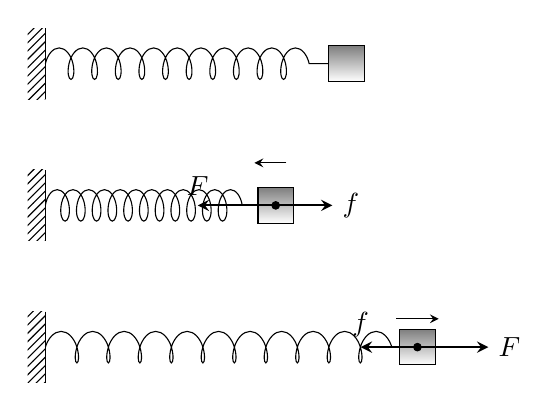
\begin{tikzpicture}[>=stealth,scale=0.9]
  \tikzstyle{spring1}=[decorate,decoration={aspect=0.5, segment length=3mm, amplitude=2mm,coil}]
  \tikzstyle{spring2}=[decorate,decoration={aspect=0.5, segment length=2mm, amplitude=2mm,coil}]
  \tikzstyle{spring3}=[decorate,decoration={aspect=0.5, segment length=4mm, amplitude=2mm,coil}]
  \fill [pattern = north east lines] (-.25,2) rectangle (0,3);
  \fill [pattern = north east lines] (-.25,0) rectangle (0,1);
  \fill [pattern = north east lines] (-.25,-1) rectangle (0,-2);
  \draw(0,2)--(0,3);  \draw(0,0)--(0,1);  \draw(0,-1)--(0,-2); 
  \draw [shade] (4, 2.25) rectangle (4.5, 2.75);
  \draw [shade] (3,.25) rectangle  (3.5, .75);
  \draw [shade] (5,-1.75) rectangle  (5.5, -1.25);
  \draw [spring1](0,2.5)--(4,2.5);
  \draw [spring2](0,.5)--(3,.5);
  \draw [spring3](0,-1.5)--(5,-1.5);
  \draw[fill=black] (6.5/2,.5) circle (1.5pt);  \draw [fill=black] (10.5/2,-1.5) circle (1.5pt);
  \draw [<->, thick]  (6.5/2+.8,.5)node[right]{$f$}-- (6.5/2-1.1,.5)node[above]{$F$};
  \draw [<->, thick]  (10.5/2+1,-1.5)node[right]{$F$}-- (10.5/2-.8,-1.5)node[above]{$f$};
  \draw [->] (6.2/2+.3, 1.1)--(6.5/2-.3, 1.1);
  \draw [->] (10.5/2-.3, -1.1)--(10.5/2+.3,-1.1);
\end{tikzpicture}
\end{document}